\documentclass[tikz,border=8pt]{standalone}
\usepackage{helvet}
\renewcommand{\familydefault}{\sfdefault}
\usetikzlibrary{decorations.pathmorphing}
\begin{document}
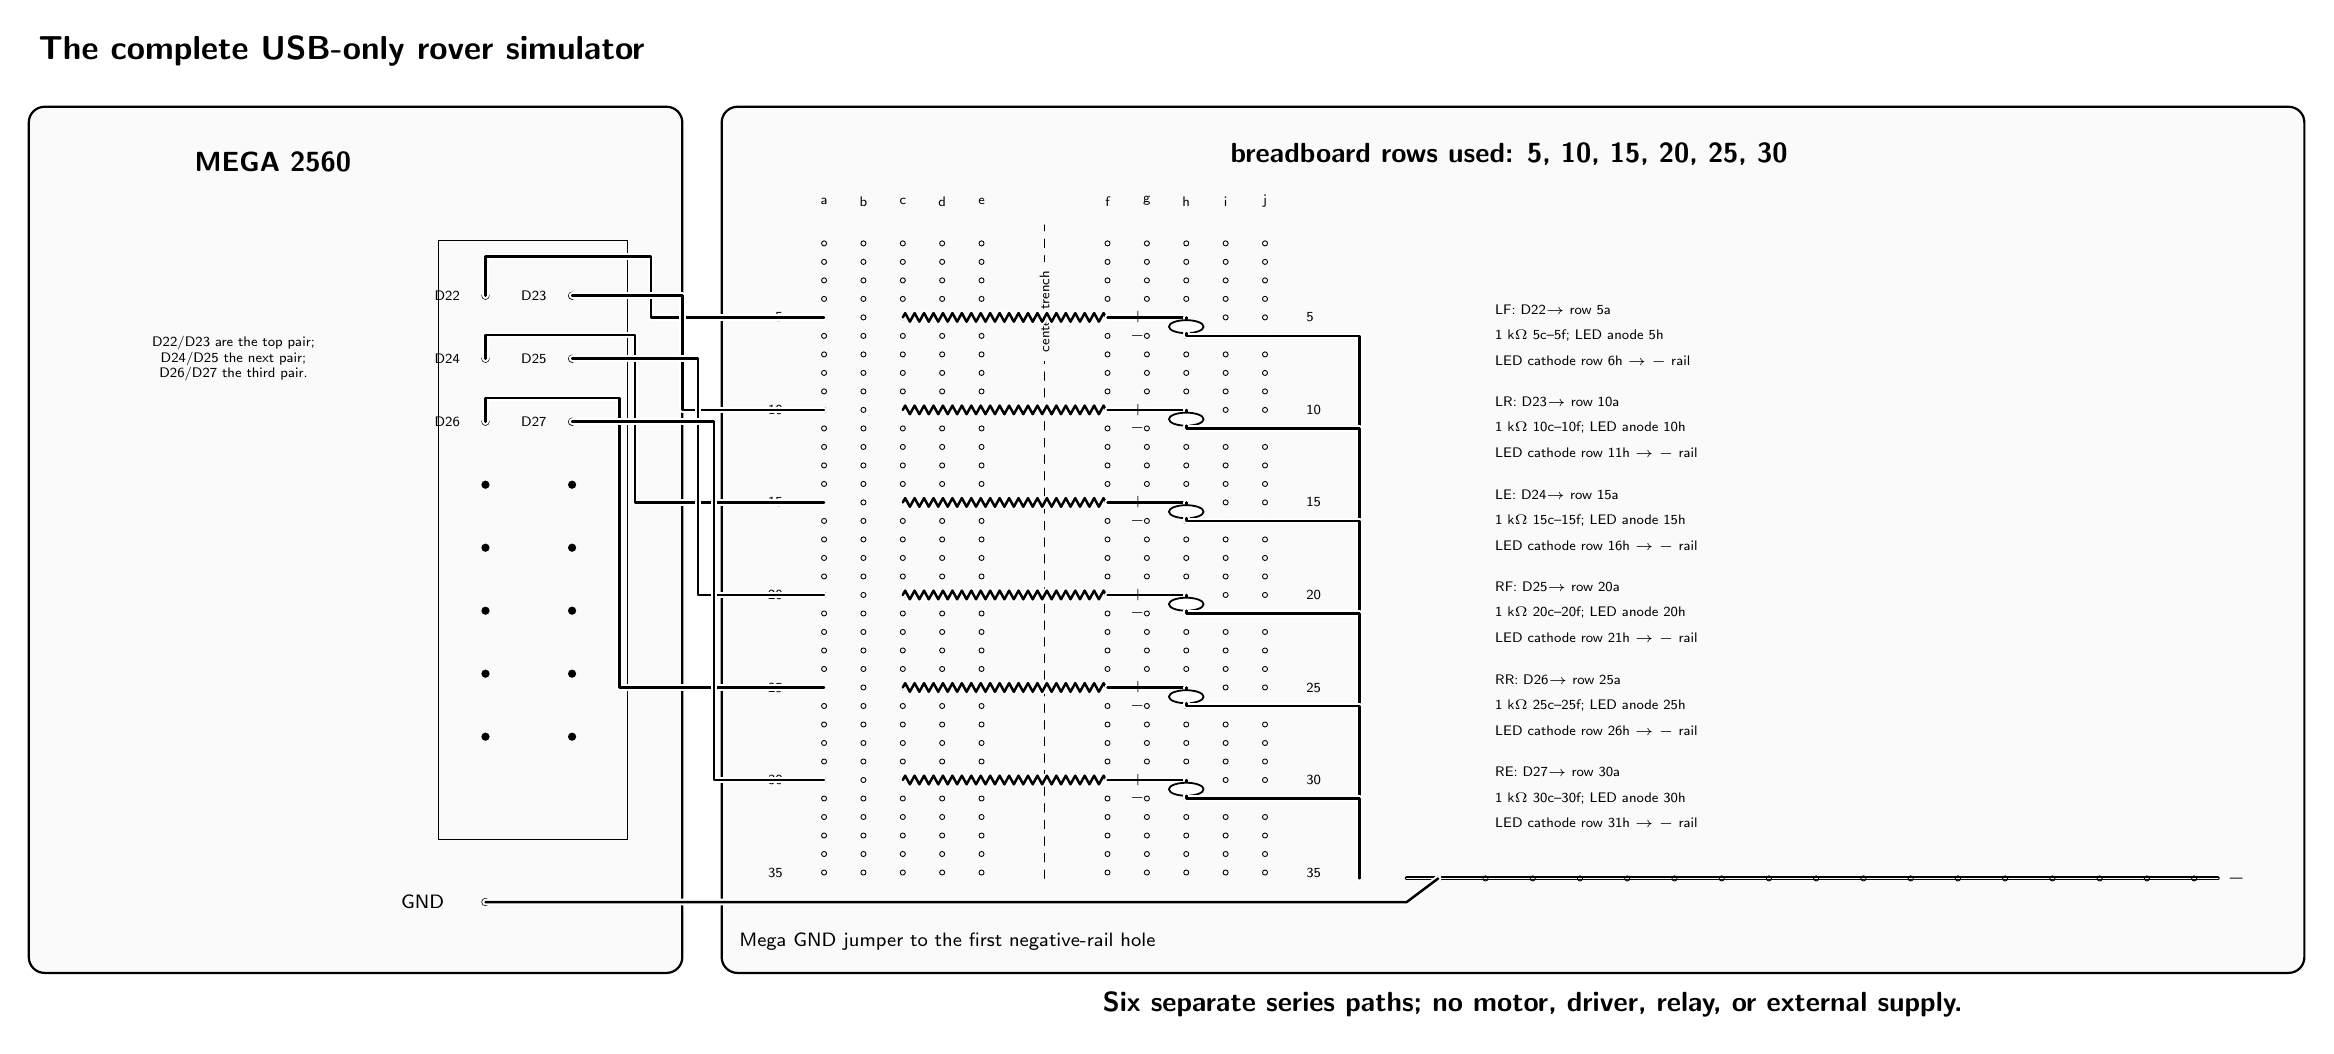
\begin{tikzpicture}[x=1mm,y=1mm,line cap=round,line join=round,
  board/.style={draw,line width=.8pt,rounded corners=2mm,fill=black!2},
  hole/.style={circle,draw,line width=.32pt,inner sep=.65pt},
  pin/.style={circle,fill=black,inner sep=1.05pt},
  wire/.style={preaction={draw=white,line width=2.4pt},line width=.9pt},
  tiny/.style={font=\fontsize{5.1}{5.7}\selectfont},
  small/.style={font=\scriptsize}]

\node[anchor=west,font=\bfseries\large] at (3,125)
  {The complete USB-only rover simulator};

% Literal Mega paired header.
\draw[board] (3,8) rectangle (86,118);
\node[font=\bfseries] at (34,111) {MEGA 2560};
\draw (55,25) rectangle (79,101);
\foreach \r in {0,...,7}
{
  \pgfmathsetmacro{\yy}{94-\r*8}
  \node[pin] at (61,\yy) {};
  \node[pin] at (72,\yy) {};
}
\foreach \p/\x/\y in {22/61/94,23/72/94,24/61/86,25/72/86,26/61/78,27/72/78}
  \node[tiny,anchor=east] at (\x-2,\y) {D\p};
\node[pin] at (61,17) {};
\node[small,anchor=east] at (57,17) {GND};
\node[tiny,align=center] at (29,86)
  {D22/D23 are the top pair;\\D24/D25 the next pair;\\D26/D27 the third pair.};

% Literal breadboard coordinate field.
\draw[board] (91,8) rectangle (292,118);
\node[small,font=\bfseries] at (191,112) {breadboard rows used: 5, 10, 15, 20, 25, 30};
\foreach \c/\x in {a/104,b/109,c/114,d/119,e/124,f/140,g/145,h/150,i/155,j/160}
  \node[tiny] at (\x,106) {\c};
\draw[dashed,line width=.45pt] (132,20) -- (132,103);
\node[tiny,rotate=90,fill=black!2] at (132,92) {center trench};
\foreach \r in {1,...,35}
{
  \pgfmathsetmacro{\yy}{103-\r*2.35}
  \foreach \x in {104,109,114,119,124,140,145,150,155,160}
    \node[hole] at (\x,\yy) {};
}
\foreach \r in {5,10,15,20,25,30,35}
{
  \pgfmathsetmacro{\yy}{103-\r*2.35}
  \node[tiny,anchor=east] at (100,\yy) {\r};
  \node[tiny,anchor=west] at (164,\yy) {\r};
}
\draw[double,line width=.4pt] (178,20) -- (281,20);
\node[small,anchor=west] at (281,20) {$-$};
\foreach \x in {182,188,...,278}
  \node[hole] at (\x,20) {};

% Six independent pin -> resistor -> LED -> ground paths.
\foreach \p/\mx/\my/\r/\name in {
  22/61/94/5/LF,
  23/72/94/10/LR,
  24/61/86/15/LE,
  25/72/86/20/RF,
  26/61/78/25/RR,
  27/72/78/30/RE}
{
  \pgfmathsetmacro{\yy}{103-\r*2.35}
  \pgfmathsetmacro{\yc}{\yy-2.35}
  \draw[wire,decorate,decoration={zigzag,segment length=1.2mm,amplitude=.55mm}]
    (114,\yy) -- (140,\yy);
  \draw[wire] (140,\yy) -- (150,\yy);
  \draw[wire] (150,\yy) -- (150,\yy-.35);
  \draw[fill=white,line width=.65pt] (150,\yy-1.175) ellipse (2.2 and .825);
  \draw[wire] (150,\yy-2) -- (150,\yc) -- (172,\yc) -- (172,20);
  \node[tiny,anchor=east] at (146,\yy) {$+$};
  \node[tiny,anchor=east] at (146,\yc) {$-$};
  \node[tiny,anchor=west] at (188,\yy+1) {\name: D\p $\rightarrow$ row \r a};
  \node[tiny,anchor=west] at (188,\yy-2.3)
    {1 k$\Omega$ \r c--\r f; LED anode \r h};
  \node[tiny,anchor=west] at (188,\yy-5.6)
    {LED cathode row \the\numexpr\r+1\relax h $\rightarrow$ $-$ rail};
}
% Fan the paired pins apart before the breadboard; no two signal wires join.
\draw[wire] (61,94) -- (61,99) -- (82,99) -- (82,91.25) -- (104,91.25);
\draw[wire] (72,94) -- (86,94) -- (86,79.50) -- (104,79.50);
\draw[wire] (61,86) -- (61,89) -- (80,89) -- (80,67.75) -- (104,67.75);
\draw[wire] (72,86) -- (88,86) -- (88,56.00) -- (104,56.00);
\draw[wire] (61,78) -- (61,81) -- (78,81) -- (78,44.25) -- (104,44.25);
\draw[wire] (72,78) -- (90,78) -- (90,32.50) -- (104,32.50);
\draw[wire] (61,17) -- (178,17) -- (182,20);
\node[small,anchor=west] at (92,12) {Mega GND jumper to the first negative-rail hole};

\node[font=\bfseries] at (194,4)
  {Six separate series paths; no motor, driver, relay, or external supply.};
\end{tikzpicture}
\end{document}
